\documentclass[12pt,a4paper,twoside]{article}
\usepackage{amsmath}
\usepackage{amssymb}
\usepackage{graphicx}

\setlength{\voffset}{-28.4mm}
\setlength{\hoffset}{-1in}
\setlength{\topmargin}{20mm}
\setlength{\oddsidemargin}{25mm}
\setlength{\evensidemargin}{25mm}
\setlength{\textwidth}{160mm}

\setlength{\parindent}{0pt}

\setlength{\textheight}{235mm}
\setlength{\footskip}{20mm}
\setlength{\headsep}{50pt}
\setlength{\headheight}{0pt}

\begin{document}
\pagestyle{empty}
%%%% Title page
\begin{titlepage}
\begin{center}

\includegraphics{assets/TUMlschwarz.png}\\[3mm]
\sf
{\Large
  Technische Universit\"at M\"unchen\\[5mm]
  Department of Mathematics\\[8mm]
}
\normalsize
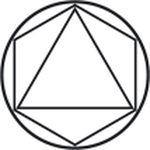
\includegraphics{assets/TUMlMschwarz.png}\\[15mm]

Bachelor's Thesis\\[15mm]

{\Huge
  Extension Complexity of convex n-gons
}
\bigskip

\normalsize

Josef Wittmann
\end{center}
\vspace*{75mm}

Supervisor: Prof. Dr. Stefan Weltge
\medskip

Advisor: ...
\medskip

Submission Date: ...

\end{titlepage}
%%%% The following has to be signed by hand!

\vspace*{150mm}

I assure the single handed composition of this bachelor's thesis only supported by declared resources.
\bigskip

Garching, 
\newpage
%%%% Zusammenfassung in deutscher Sprache
\section*{Zusammenfassung}
Bei einer in englischer Sprache verfassten Arbeit muss eine Zusammenfassung in deutscher Sprache vorangestellt werden.
Daf\"ur ist hier Platz.

\newpage
\tableofcontents
\newpage

%%%% Page numbering restarts here
\pagenumbering{arabic}
\pagestyle{headings}

\section*{Abstract}
In this paper we provide an overview of the current state of the extension complexity of convex $n$-gons (i.e., two-dimensional polytopes with $n$ vertices). First we give an overview of the lower bound  ($xc(P_n) \geq \sqrt{n}$) and summarize the arguments, why this is true. Then we provide a geometric visualization of Shitov's proof that $xc(P_n) \leq \frac{6}{7}n$. From that we give a geometric proof of Shitov's result that $xc(P_n) \leq o(n)$ from which we improve the known upper bound for the extension complexity of $n$-gons slightly.

\section{Explicit representation of the lower bound}

\section{Geometric version of Shitov's heptagon proof}

\section{Geometric proof for sublinear extension complexity and improvements}





\cite{Padrol}
\cite{HiddenVertices}
\cite{UpperBound}
\cite{Sublinear}

\bibliographystyle{plain}
\bibliography{ExtensionComplexityConvexN-Gons}

\end{document}



